% tcm-more.tex

\documentclass{standalone}

% TODO: using ``chains''
\usepackage{tikz}
\usetikzlibrary{shapes, positioning, arrows.meta, decorations.pathmorphing, chains}

\begin{document}
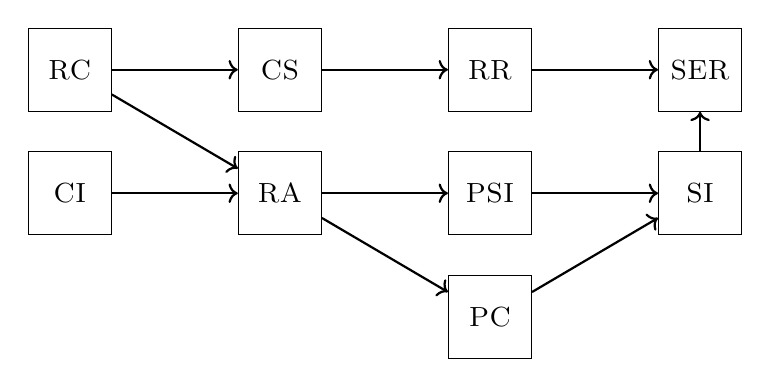
\begin{tikzpicture}[model/.style = {draw, minimum size = 30pt},
  node distance = 0.5cm and 1.6cm]

  \node[model] (rc) {\textsc{RC}};
  \node[model, right = of rc] (cs) {\textsc{CS}};
  \node[model, right = of cs] (rr) {\textsc{RR}};
  \node[model, right = of rr] (ser) {\textsc{SER}};

  \node[model, below = of rc] (ci) {\textsc{CI}};
  \node[model, right = of ci] (ra) {\textsc{RA}};
  \node[model, right = of ra] (psi) {\textsc{PSI}};
  \node[model, below = of psi] (pc) {\textsc{PC}};
  \node[model, right = of psi] (si) {\textsc{SI}};

  \path[every edge, ->, thick] (rc) edge (cs) edge (ra)
     (cs) edge (rr)
     (rr) edge (ser)
     (ci) edge (ra)
     (ra) edge (psi) edge (pc)
     (pc) edge (si)
     (psi) edge (si)
     (si) edge (ser);
\end{tikzpicture}
\end{document}